% ===========================================================================
% MODELO DE RELATORIO  ·  ENE0046 Laboratorio de Eletronica  ·  2026/2
%
% Como usar
%   1. Preencha o bloco IDENTIFICACAO logo abaixo.
%   2. Deixe comentados os autores que nao existirem. Um autor fica centralizado,
%      dois dividem a linha, tres ocupam tercos.
%   3. Substitua o texto de cada secao pelo seu. As orientacoes que estao la
%      dizem o que se espera em cada uma.
%   4. Compile com pdflatex duas vezes, ou com latexmk -pdf.
%
% Estrutura
%   Roteiro 1 nao tem bancada: use so a subsecao 4.1 e a 5.1, e compare o calculo
%   analitico com a simulacao de projeto.
%   Roteiros 2 a 7 usam a estrutura inteira.
%
% O arquivo estilo-relatorio.tex deve estar na mesma pasta deste arquivo. A logo
% e as figuras ficam organizadas na subpasta imgs/, como no relatorio preenchido.
% ===========================================================================
\documentclass[11pt,a4paper]{article}
% !TeX root = modelo-relatorio.tex
% Formatacao do relatorio. Compile o modelo-relatorio.tex, nao este arquivo.
\usepackage[T1]{fontenc}
\usepackage[utf8]{inputenc}
\usepackage[brazil]{babel}
\usepackage[a4paper,top=1.6cm,bottom=1.8cm,left=2.1cm,right=2.1cm]{geometry}
\usepackage[default]{lato}
\usepackage{amsmath,amssymb}
\usepackage{siunitx}
\usepackage{graphicx}
\usepackage{booktabs,array,longtable,colortbl}
\usepackage{enumitem}
\usepackage{tcolorbox}
\usepackage{xcolor}
\usepackage{tikz}
\usepackage{titlesec}
\usepackage{fancyhdr}
\usepackage{caption}
\usepackage{etoolbox}
\usepackage[colorlinks=true,linkcolor=azul,urlcolor=azul,citecolor=azul]{hyperref}
\tcbuselibrary{skins,breakable}

\definecolor{azul}{HTML}{0A4B8C}
\definecolor{azulclaro}{HTML}{E8F0F8}
\definecolor{verde}{HTML}{0B7A4B}
\definecolor{cinza}{HTML}{5B6672}
\definecolor{cinzaclaro}{HTML}{F4F6F8}
\definecolor{vinho}{HTML}{B04A4A}
\definecolor{vinhoclaro}{HTML}{FBF2F2}

\sisetup{output-decimal-marker={,}, per-mode=symbol}
\setlength{\parindent}{0pt}
\setlength{\parskip}{6pt plus 1pt}
\setlist{itemsep=3pt, topsep=4pt, parsep=0pt, leftmargin=1.3em}
\renewcommand{\arraystretch}{1.25}
\linespread{1.06}

% ---- secoes numeradas com marcador colorido -------------------------------
\titleformat{\section}[hang]
  {\Large\bfseries\color{azul}}
  {\raisebox{-1pt}{\tikz\node[fill=azul,text=white,rounded corners=2pt,
     inner sep=3pt,minimum width=20pt,align=center]{\bfseries\thesection};}}
  {10pt}{}
\titlespacing*{\section}{0pt}{16pt plus 3pt}{6pt}
\titleformat{\subsection}{\large\bfseries\color{cinza}}{\thesubsection}{8pt}{}
\titlespacing*{\subsection}{0pt}{11pt plus 2pt}{3pt}

% ---- legendas -------------------------------------------------------------
\captionsetup{font=small,labelfont={bf,color=azul},labelsep=period,skip=6pt}

% ---- identificacao --------------------------------------------------------
\newcommand{\autorA}{}\newcommand{\matA}{}
\newcommand{\autorB}{}\newcommand{\matB}{}
\newcommand{\autorC}{}\newcommand{\matC}{}
\newcommand{\autorum}[2]{\renewcommand{\autorA}{#1}\renewcommand{\matA}{#2}}
\newcommand{\autordois}[2]{\renewcommand{\autorB}{#1}\renewcommand{\matB}{#2}}
\newcommand{\autortres}[2]{\renewcommand{\autorC}{#1}\renewcommand{\matC}{#2}}

\newcommand{\disciplina}{ENE0046 · Laboratório de Eletrônica}
\newcommand{\semestre}{2026/2}
\newcommand{\turma}{}
\newcommand{\roteironum}{}
\newcommand{\roteirotema}{}
\newcommand{\aturma}[1]{\renewcommand{\turma}{#1}}
\newcommand{\roteiro}[2]{\renewcommand{\roteironum}{#1}\renewcommand{\roteirotema}{#2}}

\newcommand{\umautor}[2]{%
  \begin{minipage}[t]{\dimexpr\linewidth-4pt\relax}\centering
    \parbox[t][30pt][t]{\linewidth}{\centering
      {\fontsize{10.5}{12.5}\selectfont #1}}\\[-2pt]
    {\color{cinza}\fontsize{9}{11}\selectfont\texttt{#2}}
  \end{minipage}}

\newcounter{nautores}
\newcommand{\blocoautores}{%
  \setcounter{nautores}{0}%
  \ifdefempty{\autorA}{}{\stepcounter{nautores}}%
  \ifdefempty{\autorB}{}{\stepcounter{nautores}}%
  \ifdefempty{\autorC}{}{\stepcounter{nautores}}%
  \ifnum\value{nautores}=0
    \begin{center}\color{vinho}\bfseries
      Preencha ao menos um autor no preâmbulo do arquivo.
    \end{center}
  \else
    \begin{center}
    \ifcase\value{nautores}\or
      % --- um autor: ocupa o centro
      \begin{minipage}{0.5\textwidth}\umautor{\autorA}{\matA}\end{minipage}%
    \or
      % --- dois autores: metades
      \begin{minipage}{0.42\textwidth}\umautor{\autorA}{\matA}\end{minipage}\hspace{0.04\textwidth}%
      \begin{minipage}{0.42\textwidth}\umautor{\autorB}{\matB}\end{minipage}%
    \or
      % --- tres autores: tercos
      \begin{minipage}{0.31\textwidth}\umautor{\autorA}{\matA}\end{minipage}\hspace{0.015\textwidth}%
      \begin{minipage}{0.31\textwidth}\umautor{\autorB}{\matB}\end{minipage}\hspace{0.015\textwidth}%
      \begin{minipage}{0.31\textwidth}\umautor{\autorC}{\matC}\end{minipage}%
    \fi
    \end{center}
  \fi}

% ---- cabecalho do relatorio -----------------------------------------------
\newcommand{\capa}{%
\begin{tcolorbox}[colback=azul,colframe=azul,boxrule=0pt,arc=4pt,
  left=16pt,right=16pt,top=13pt,bottom=13pt]
\color{white}
\begin{minipage}{0.76\textwidth}
  {\fontsize{9}{11}\selectfont\textbf{\MakeUppercase{\disciplina{} · \semestre{}}}}\\[6pt]
  {\fontsize{22}{25}\selectfont\bfseries Relatório do Roteiro \roteironum}\\[3pt]
  {\fontsize{12.5}{15}\selectfont \roteirotema}
\end{minipage}\hfill
\begin{minipage}{0.2\textwidth}\raggedleft
  \colorbox{white}{\hspace{2pt}\raisebox{-2pt}{
\includegraphics[height=30pt]{imgs/logo-unb.png}}\hspace{2pt}}
\end{minipage}
\end{tcolorbox}
\vspace{10pt}
\blocoautores
\ifdefempty{\turma}{}{%
  \begin{center}{\color{cinza}\fontsize{9}{11}\selectfont Turma \turma}\end{center}}
\vspace{4pt}
{\color{azulclaro}\hrule height 2pt}
\vspace{2pt}}

% ---- caixas auxiliares ----------------------------------------------------
\newtcolorbox{formula}{colback=azulclaro,colframe=azul,boxrule=0.8pt,arc=3pt,
  left=12pt,right=12pt,top=9pt,bottom=9pt}
\newtcolorbox{nota}[1]{colback=cinzaclaro,colframe=cinza,boxrule=0.8pt,arc=3pt,
  left=10pt,right=10pt,top=7pt,bottom=7pt,
  title={\textbf{#1}},fonttitle=\small\bfseries,coltitle=white,colbacktitle=cinza}
\newenvironment{resumo}
  {\vspace{6pt}\begin{center}\begin{minipage}{0.92\textwidth}
   \begin{tcolorbox}[colback=cinzaclaro,colframe=cinzaclaro,boxrule=0pt,arc=3pt,
     left=14pt,right=14pt,top=10pt,bottom=10pt,
     borderline west={2.5pt}{0pt}{azul}]
   {\color{azul}\fontsize{8}{10}\selectfont\textbf{RESUMO}}\\[4pt]
   \small}
  {\end{tcolorbox}\end{minipage}\end{center}\vspace{2pt}}

\newtcolorbox{espec}{colback=azulclaro,colframe=azul,boxrule=0.8pt,arc=3pt,
  left=12pt,right=12pt,top=9pt,bottom=9pt,
  title={\textbf{Especificação da matrícula}},fonttitle=\bfseries,
  coltitle=white,colbacktitle=azul}

\newtcolorbox{especbancada}{colback=azulclaro,colframe=azul,boxrule=0.8pt,arc=3pt,
  left=12pt,right=12pt,top=9pt,bottom=9pt,
  title={\textbf{Especificação da Equipe}},fonttitle=\bfseries,
  coltitle=white,colbacktitle=azul}

% ---- rodape ---------------------------------------------------------------
\pagestyle{fancy}\fancyhf{}
\renewcommand{\headrulewidth}{0pt}
\renewcommand{\footrulewidth}{0.4pt}
\fancyfoot[L]{\color{cinza}\fontsize{8}{10}\selectfont \disciplina{} · \semestre{} · Roteiro \roteironum}
\fancyfoot[R]{\color{cinza}\fontsize{8}{10}\selectfont \thepage}

\newlist{referencias}{itemize}{1}
\setlist[referencias]{label={}, leftmargin=1.1em, itemindent=-1.1em,
                     itemsep=3pt, topsep=2pt, parsep=0pt}

\newcommand{\mat}[1]{\texttt{\textbf{#1}}}


% --------------------------- IDENTIFICACAO ---------------------------------
\roteiro{1}{Simulação de Circuitos: Introdução ao LTspice}
\aturma{03}

\autorum{Lurian Correia Lima}{22/2005395} 
\autordois{Guilherme Cardoso Oliveira da Silva Júnior}{23/1038626}
\autortres{Daniel Campos Silva}{23/1036775}
% ---------------------------------------------------------------------------

\begin{document}
\capa

\begin{resumo}
% Escreva este parágrafo por último, com 100 a 150 palavras. Diga o que você projetou, sob
% qual especificação, o que simulou ou mediu, o principal resultado numérico e a que
% conclusão chegou. Quem ler só este parágrafo deve saber o que você fez e o que encontrou.
\end{resumo}

\section{Introdução}

% Comece pelo problema, e não pelo circuito. Que necessidade de engenharia deu origem a esta
% topologia, onde você a encontraria em um equipamento real e o que aconteceria sem ela. Duas
% ou três referências ajudam aqui.

% Depois estreite o foco: que aspecto você vai investigar, sob quais condições, e por que
% vale a pena verificá-lo. Se o roteiro impõe alguma restrição de projeto que parece
% arbitrária, aproveite para explicar a razão dela.

% No último parágrafo, diga qual é o objetivo deste relatório e como o texto está
% organizado, seção a seção.

\section{Fundamentação teórica}

% Deduza as expressões que você vai usar mais adiante, partindo das leis de circuito.
% Numere as equações que forem retomadas no restante do texto.

% \begin{equation}
% H(j\omega) = \frac{1}{1+j\omega RC}
% \label{eq:exemplo}
% \end{equation}

% Toda grandeza que aparecer nos resultados precisa ter sido apresentada aqui. Explique o que
% cada termo significa fisicamente, não apenas o que a letra representa. Registre as hipóteses
% que você está assumindo, como linearidade ou idealidade dos componentes: se alguma delas
% não se sustentar no experimento, você vai retomá-la na discussão.

% Se o circuito tiver regimes de funcionamento distintos, apresente cada um e diga o que os
% separa.

\section{Especificação e projeto}

% Transcreva os parâmetros que a sua matrícula determina, mostrando a conta a partir dos
% dígitos.

% \begin{espec}
% Matrícula \mat{00/0000000}. \\
% Preencha aqui os parâmetros calculados a partir dos dígitos, conforme o roteiro.
% \end{espec}

% Leve cada parâmetro até o valor de componente, deixando visível a expressão que você
% inverteu para chegar lá. Depois escolha o valor na série comercial e calcule o quanto essa
% escolha afasta você do valor ideal. A tabela abaixo organiza isso, e é ela que depois
% permite separar o que veio do projeto do que veio da montagem.

% \begin{center}
% \begin{tabular}{@{}lrrr@{}}
% \toprule
% \textbf{Grandeza} & \textbf{Teórico} & \textbf{Adotado} & \textbf{Desvio} \\
% \midrule
% & & & \\
% \bottomrule
% \end{tabular}
% \end{center}

% Se mais de uma combinação atender à especificação, diga por que escolheu esta, mostrando
% que as outras ficavam mais distantes.

\section{Metodologia}

% Conte o que você fez e com quais parâmetros, de modo que um colega consiga repetir sem
% precisar perguntar nada. Explique as escolhas que não são evidentes: por que essa faixa de
% varredura, por que esse passo de integração, por que esse intervalo de gravação.

% Inclua a figura do esquemático, com legenda que descreva o que ela mostra, e cite-a no
% texto, como na Figura~\ref{fig:exemplo}. Se uma figura não for mencionada em nenhum
% parágrafo, ela provavelmente não precisa estar aqui.

\subsection{Simulação de projeto, uma por integrante}

% Cada integrante recebeu uma especificação diferente da própria matrícula, e portanto chegou
% a um dimensionamento diferente. Traga aqui \textbf{uma simulação por integrante}, cada uma
% com os componentes que aquela pessoa projetou. São elas que mostram se cada projeto cumpre
% o que foi pedido.

```latex
\subsection{Montagem em bancada}

A montagem experimental foi realizada conforme a especificação da equipe 2, apresentada na Seção 4.1 do roteiro. Nessa configuração, a fonte senoidal foi ajustada para uma tensão de $20\,\text{V}_{pp}$, frequência de $60\,\text{Hz}$ e carga de alta impedância no gerador de funções. Portanto, a tensão de pico nominal da entrada era de $10\,\text{V}$. A carga utilizada foi um resistor nominal de $4{,}7\,\text{k}\Omega$, correspondente à corrente de aproximadamente $1{,}4\,\text{mA}$ quando submetido à tensão de referência de $6{,}8\,\text{V}$ estabelecida pelo roteiro.

Antes de iniciar as montagens, os componentes foram medidos individualmente, conforme solicitado no procedimento experimental. O resistor de carga apresentou resistência de $4{,}688\,\text{k}\Omega$, valor ligeiramente inferior ao nominal de $4{,}7\,\text{k}\Omega$. Os capacitores utilizados apresentaram capacitâncias de $48{,}8\,\mu\text{F}$ e $4{,}84\,\mu\text{F}$, respectivamente. Esses valores medidos foram considerados na análise dos resultados, uma vez que a capacitância efetiva influencia diretamente o ripple observado na saída dos retificadores com filtro.

O capacitor de $48{,}8\,\mu\text{F}$ foi empregado como capacitor principal de filtro, enquanto o componente de $4{,}84\,\mu\text{F}$ foi utilizado na montagem de comparação. A escolha do capacitor principal é coerente com o dimensionamento teórico: para uma corrente de carga de $1{,}4\,\text{mA}$, frequência de retificação de $60\,\text{Hz}$ e ripple máximo de $1{,}5\,\text{V}_{pp}$, a aproximação da Equação~(1) fornece

\[
C_{\mathrm{calc}} =
\frac{I_L}{fV_r}
=
\frac{1{,}4\times10^{-3}}
{60\times1{,}5}
\approx 15{,}56\,\mu\text{F}.
\]

Assim, entre os capacitores previstos para a bancada, selecionou-se o de $47\,\mu\text{F}$, cujo valor medido foi $48{,}8\,\mu\text{F}$. O capacitor de comparação, medido em $4{,}84\,\mu\text{F}$, permite avaliar experimentalmente o aumento do ripple quando a capacitância é reduzida aproximadamente por um fator de dez.

Durante todo o experimento, foram observadas as recomendações de conexão dos instrumentos descritas na Seção 4.2 do roteiro. O terra do gerador de funções e as garras de referência do osciloscópio estão eletricamente conectados. Por isso, nas montagens de meia onda, os canais do osciloscópio foram utilizados para observar simultaneamente a tensão de entrada e a tensão na carga. Já nas montagens com ponte retificadora, a medição foi realizada somente na saída, mantendo a garra de terra na referência da carga e sem conectar outra ponta do osciloscópio diretamente aos terminais do gerador. Esse procedimento evita o curto-circuito de um dos diodos da ponte por meio do aterramento comum dos instrumentos.

\paragraph{Retificador de meia onda sem filtro.}

A primeira montagem foi constituída pelo gerador de funções, por um diodo retificador 1N4007 e pelo resistor de carga $R_L$. O diodo foi conectado em série com a carga e orientado para permitir a condução durante os semiciclos positivos da tensão de entrada. Durante os semiciclos negativos, o componente permanece reversamente polarizado e bloqueia a corrente, fazendo com que a tensão na carga fique próxima de zero.

A Figura~\ref{fig:montagem_meia_onda} apresenta a montagem experimental do retificador de meia onda sem capacitor. Nessa configuração, o primeiro canal do osciloscópio foi utilizado para observar a tensão do gerador, enquanto o segundo canal foi conectado à carga. Foram registrados os valores de pico dos dois sinais e a tensão média na saída, esta última obtida com o multímetro.

\begin{figure}[htbp]
    \centering
    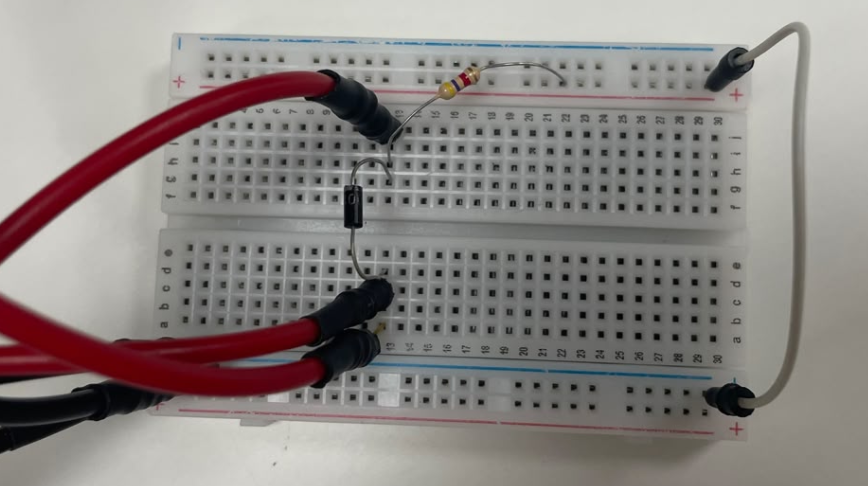
\includegraphics[width=0.85\textwidth]
    {imgs/montagem/retificador_de_meia_onda_montagem.png}
    \caption{Montagem em bancada do retificador de meia onda sem filtro capacitivo.}
    \label{fig:montagem_meia_onda}
\end{figure}

O pico medido na entrada foi de $9{,}6\,\text{V}$, ligeiramente inferior aos $10\,\text{V}$ nominais. Na carga, o pico foi de $9{,}2\,\text{V}$, resultando em uma diferença de $0{,}4\,\text{V}$ entre a entrada e a saída. Essa diferença corresponde à queda de tensão efetiva observada no diodo durante a condução, nas condições de corrente do experimento. A tensão média medida na carga foi de $2{,}928\,\text{V}$, valor inferior à aproximação ideal de $V_p/\pi \approx 3{,}18\,\text{V}$ calculada com o pico nominal de $10\,\text{V}$.

\paragraph{Retificador de meia onda com filtro capacitivo.}

Na segunda montagem, foi acrescentado o capacitor de $48{,}8\,\mu\text{F}$ em paralelo com o resistor de carga. O terminal negativo do capacitor eletrolítico foi conectado à referência do circuito, respeitando sua polaridade. Durante a subida da tensão de entrada, o diodo conduz nas proximidades do pico e carrega o capacitor. Quando a tensão da fonte diminui, o diodo deixa de conduzir e o capacitor passa a fornecer corrente à carga, descarregando-se gradualmente até o próximo pico.

A Figura~\ref{fig:montagem_meia_onda_filtro} apresenta a montagem com o capacitor de filtro principal. O ripple foi medido com o canal 2 do osciloscópio em acoplamento AC, utilizando os cursores para determinar a diferença entre os valores máximo e mínimo da ondulação. A tensão contínua na carga foi obtida com o multímetro.

\begin{figure}[htbp]
    \centering
    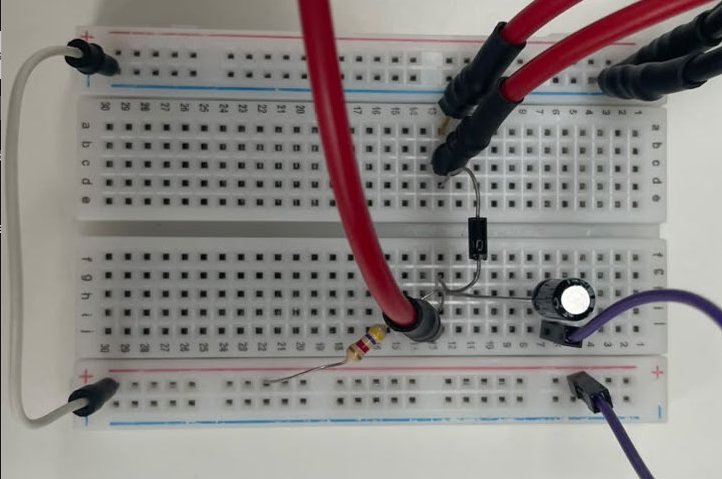
\includegraphics[width=0.85\textwidth]
    {imgs/montagem/retificador_de_meia_onda_com_filtro_projeto_montagem.png}
    \caption{Montagem em bancada do retificador de meia onda com o capacitor de filtro principal.}
    \label{fig:montagem_meia_onda_filtro}
\end{figure}

O ripple medido foi de $0{,}56\,\text{V}_{pp}$, enquanto a simulação registrou $0{,}60\,\text{V}_{pp}$. A tensão contínua medida foi de $8{,}254\,\text{V}$. A ondulação relativamente pequena em comparação com a tensão média evidencia o efeito de armazenamento de energia do capacitor, que sustenta a alimentação da carga durante o intervalo em que o diodo permanece bloqueado.

Em seguida, o capacitor principal foi substituído pelo componente de $4{,}84\,\mu\text{F}$, mantendo-se as demais condições da montagem. Essa configuração foi utilizada para avaliar a influência da capacitância sobre a descarga entre os picos da tensão retificada.

\begin{figure}[htbp]
    \centering
    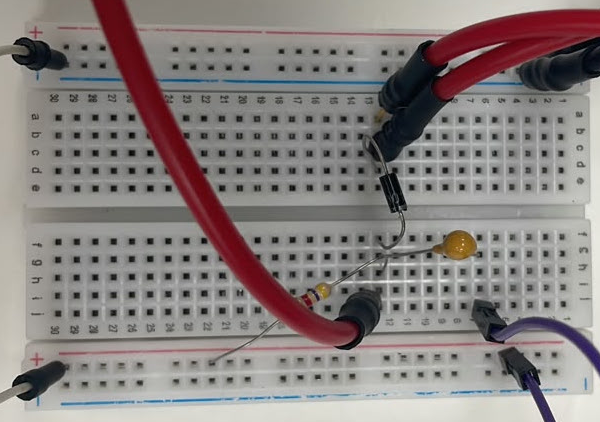
\includegraphics[width=0.85\textwidth]
    {imgs/montagem/retificador_de_meia_onda_com_filtro_comparacao_montagem.png}
    \caption{Montagem em bancada do retificador de meia onda com o capacitor de comparação.}
    \label{fig:montagem_meia_onda_comparacao}
\end{figure}

Com o capacitor menor, o ripple medido aumentou para $4{,}16\,\text{V}_{pp}$, em comparação com os $0{,}56\,\text{V}_{pp}$ obtidos com o capacitor principal. A tensão contínua medida diminuiu para $7{,}038\,\text{V}$. Esse comportamento é compatível com a relação inversa entre capacitância e ripple: quanto menor a capacitância, maior a variação de tensão durante a descarga do capacitor pela carga.

\paragraph{Ponte retificadora sem filtro.}

Na terceira configuração, o retificador de meia onda foi substituído por uma ponte formada por quatro diodos 1N4007, mantendo-se o resistor de carga e retirando-se o capacitor. Os diodos foram conectados de modo que dois conduzissem em cada semiciclo da fonte, garantindo que a corrente atravessasse a carga sempre no mesmo sentido. Nos semiciclos positivos, um par de diodos conduz; nos negativos, o outro par assume a condução.

A Figura~\ref{fig:montagem_ponte} apresenta a ponte retificadora montada em bancada. Diferentemente das configurações de meia onda, a tensão foi observada somente na saída da ponte, com a garra de terra do osciloscópio conectada à referência da carga. Essa precaução é necessária porque a referência da carga não coincide com nenhum dos terminais da fonte alternada. A conexão simultânea de uma ponta do osciloscópio ao gerador poderia aterrar indevidamente um dos terminais da ponte e provocar um curto-circuito em um diodo.

\begin{figure}[htbp]
    \centering
    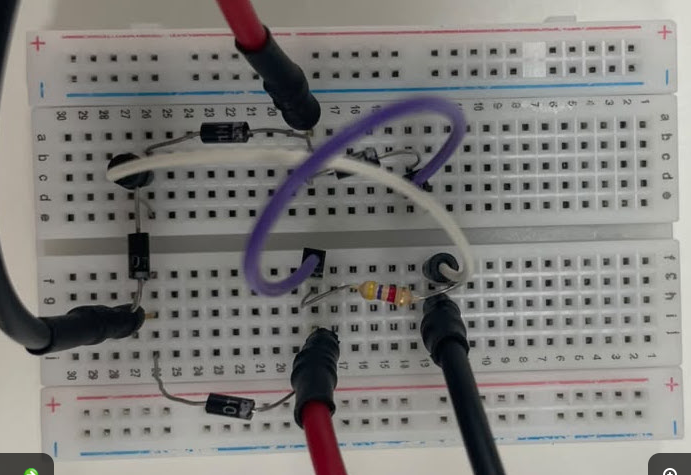
\includegraphics[width=0.85\textwidth]
    {imgs/montagem/ponte_retificadora_sem_filtro_montagem.png}
    \caption{Montagem em bancada da ponte retificadora sem filtro capacitivo.}
    \label{fig:montagem_ponte}
\end{figure}

O pico medido na saída foi de $8{,}4\,\text{V}$, inferior aos $10\,\text{V}$ nominais da fonte. Considerando o valor nominal da entrada, a diferença entre o pico da fonte e o pico da saída foi de $1{,}6\,\text{V}$. Essa diferença é maior que a observada no retificador de meia onda porque a corrente atravessa dois diodos em série durante cada semiciclo. A frequência dos picos medida foi de $119\,\text{Hz}$, próxima do valor teórico de $120\,\text{Hz}$, uma vez que a ponte retifica ambos os semiciclos da fonte de $60\,\text{Hz}$.

\paragraph{Ponte retificadora com filtro capacitivo.}

Na quarta configuração, foi conectado o capacitor de $48{,}8\,\mu\text{F}$ em paralelo com a carga da ponte retificadora, com o terminal negativo ligado à referência da saída. O princípio de funcionamento é semelhante ao da montagem de meia onda com filtro: o capacitor é carregado próximo aos picos da tensão retificada e fornece corrente à carga entre esses instantes. Entretanto, como a ponte utiliza os dois semiciclos da entrada, o intervalo entre os picos é menor e a frequência de recarga é aproximadamente duas vezes maior.

A Figura~\ref{fig:montagem_ponte_filtro} apresenta a montagem utilizada para medir o ripple e a tensão contínua na saída. Além dessas grandezas, foi determinada a tensão mínima do filtro, necessária para dimensionar o resistor em série do regulador zener.

\begin{figure}[htbp]
    \centering
    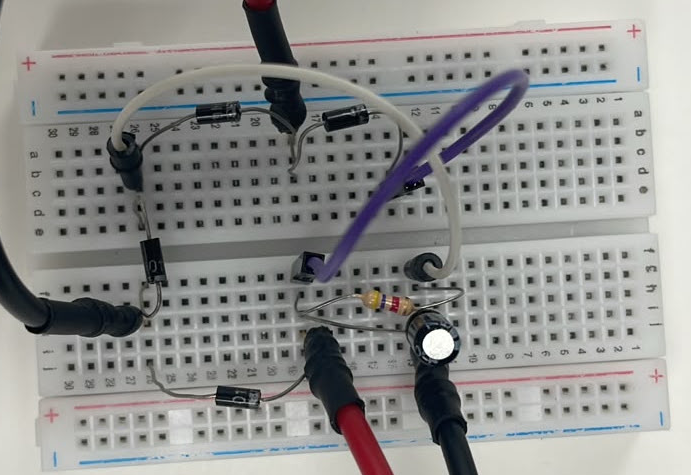
\includegraphics[width=0.85\textwidth]
    {imgs/montagem/ponte_retificadora_com_filtro_montagem.png}
    \caption{Montagem em bancada da ponte retificadora com filtro capacitivo.}
    \label{fig:montagem_ponte_filtro}
\end{figure}

O ripple medido nessa configuração foi de $0{,}26\,\text{V}_{pp}$, enquanto a tensão contínua na saída foi de $8{,}004\,\text{V}$. A tensão mínima estimada do filtro foi calculada a partir da tensão contínua e de metade do ripple:

\[
V_{\min} \approx V_{\mathrm{CC}}-\frac{V_r}{2}
=8{,}004-\frac{0{,}26}{2}
=7{,}874\,\text{V}.
\]

O ripple obtido foi inferior ao observado com o mesmo capacitor no retificador de meia onda, conforme esperado pela duplicação da frequência dos picos de recarga.

\paragraph{Regulação com diodo zener.}

Na última configuração, foi acrescentado um resistor em série entre a saída do filtro e a carga, além do diodo zener conectado em paralelo com a carga. O resistor limita a corrente fornecida pelo retificador, enquanto o zener, polarizado reversamente, mantém a tensão de saída aproximadamente constante quando opera na região de ruptura e recebe corrente suficiente.

O dimensionamento de $R_S$ deve considerar a tensão mínima do filtro e a corrente mínima exigida para a condução do zener. De acordo com a Equação~(2) do roteiro,

\[
R_S=\frac{V_{\min}-V_Z}{I_L+I_{Z,\min}}.
\]

Utilizando o valor medido de $V_{\min}=7{,}874\,\text{V}$, a tensão nominal de $6{,}8\,\text{V}$ indicada no roteiro, a corrente de carga de $1{,}4\,\text{mA}$ e a corrente mínima de zener de $1\,\text{mA}$, obtém-se aproximadamente $447{,}5\,\Omega$. O resistor disponível imediatamente inferior na série considerada para a bancada é de $390\,\Omega$. O resistor efetivamente registrado na planilha apresentou resistência de $386{,}5\,\Omega$.

\begin{figure}[htbp]
    \centering
    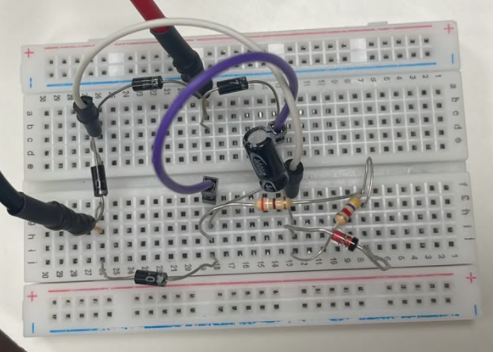
\includegraphics[width=0.85\textwidth]
    {imgs/montagem/regulacao_zener_com_carga.png}
    \caption{Montagem em bancada do regulador zener com a carga conectada.}
    \label{fig:montagem_zener_carga}
\end{figure}

Com a carga conectada, a planilha registra tensão contínua de $5{,}6\,\text{V}$ e ripple de $0{,}02\,\text{V}_{pp}$. O ripple antes do regulador era de $0{,}26\,\text{V}_{pp}$, de modo que a redução registrada corresponde a aproximadamente $92{,}3\%$. A tensão de saída permaneceu praticamente constante, indicando a atenuação da ondulação pelo regulador nas condições ensaiadas.

Por fim, a carga foi retirada, mantendo-se o regulador conectado, para verificar a tensão de saída sem consumo pela carga e avaliar a condição de maior corrente no zener. A tensão contínua registrada nessa condição foi de $5{,}604\,\text{V}$.

\begin{figure}[htbp]
    \centering
    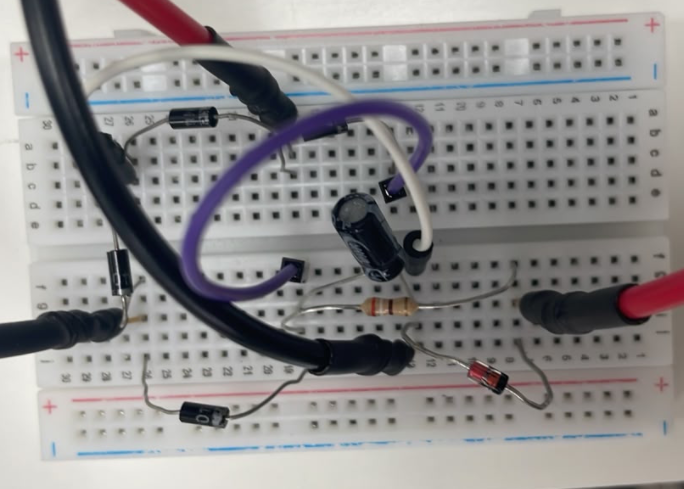
\includegraphics[width=0.85\textwidth]
    {imgs/montagem/regulacao_zener_sem_carga.png}
    \caption{Montagem em bancada do regulador zener com a carga retirada.}
    \label{fig:montagem_zener_sem_carga}
\end{figure}

É necessário destacar uma divergência na identificação do zener: o roteiro especifica o 1N754, com tensão nominal de $6{,}8\,\text{V}$, enquanto a planilha registra $5{,}6\,\text{V}$ tanto na simulação quanto nas medições de saída. Portanto, a identificação do componente utilizado deve ser conferida antes de atribuir a tensão obtida à característica nominal do 1N754. Os valores registrados são apresentados como medidos, sem presumir que correspondam a um zener de $6{,}8\,\text{V}$.

\subsection{Simulação da montagem}

As simulações desta etapa têm como objetivo reproduzir, no LTspice, as condições efetivamente utilizadas em bancada. Diferentemente da simulação de projeto, na qual os componentes são selecionados a partir dos valores calculados e nominais, a simulação da montagem deve utilizar os valores medidos dos componentes físicos. Dessa maneira, a comparação entre os resultados simulados e experimentais permite investigar a influência das tolerâncias dos componentes e das condições reais de operação.

Foram consideradas as condições de alimentação especificadas para a equipe 2: fonte senoidal de $60\,\text{Hz}$ e $20\,\text{V}_{pp}$, correspondente a um pico nominal de $10\,\text{V}$, e carga de aproximadamente $4{,}7\,\text{k}\Omega$. Nas montagens com filtro, foram utilizados os valores medidos de $48{,}8\,\mu\text{F}$ e $4{,}84\,\mu\text{F}$. Na montagem regulada, o resistor em série medido foi de $386{,}5\,\Omega$.

As análises transientes foram utilizadas para observar as formas de onda de entrada e saída, a condução dos diodos, a ondulação da tensão retificada e o comportamento do regulador. As leituras foram consideradas após o período inicial de carga do capacitor, de acordo com a recomendação do roteiro. A seguir, os resultados são apresentados por configuração.

\paragraph{Retificador de meia onda sem filtro.}

A Figura~\ref{fig:sim_meia_onda} apresenta a simulação do retificador de meia onda sem filtro. O circuito é constituído pela fonte senoidal, pelo diodo 1N4007 e pela resistência de carga. Durante o semiciclo positivo, o diodo conduz quando a tensão de entrada supera a tensão direta necessária para polarizá-lo; durante o semiciclo negativo, o diodo permanece bloqueado.

\begin{figure}[htbp]
    \centering
    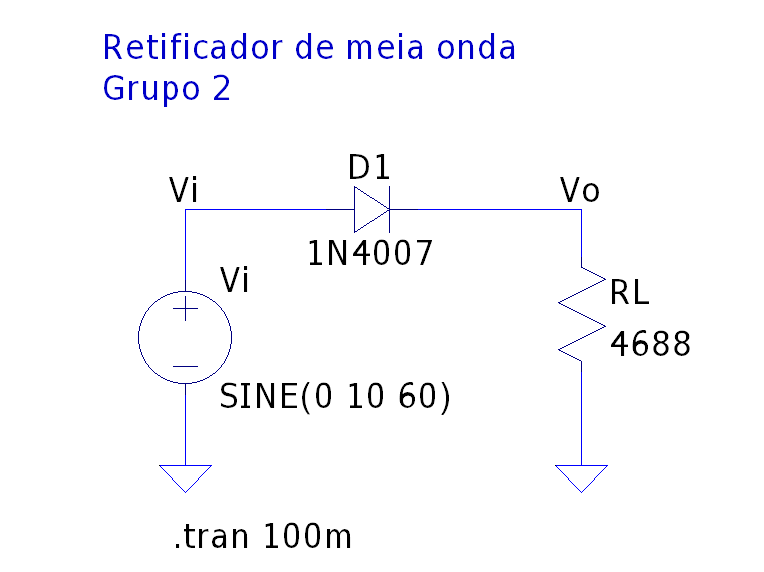
\includegraphics[width=0.85\textwidth]
    {imgs/simulacao/retificador_de_meia_onda.png}
    \caption{Simulação LTspice do retificador de meia onda sem filtro.}
    \label{fig:sim_meia_onda}
\end{figure}

O pico simulado na entrada foi de $10{,}0\,\text{V}$, enquanto o pico na carga foi de $9{,}3\,\text{V}$. Assim, a queda de tensão estimada no diodo foi de $0{,}7\,\text{V}$. O valor médio simulado na carga foi de $3{,}18\,\text{V}$, compatível com a aproximação teórica para um retificador ideal de meia onda, $V_{\mathrm{médio}}\approx V_p/\pi$.

Na bancada, foram medidos picos de $9{,}6\,\text{V}$ na entrada e $9{,}2\,\text{V}$ na carga. A queda observada entre os picos foi, portanto, de $0{,}4\,\text{V}$, enquanto a tensão média registrada foi de $2{,}928\,\text{V}$. A diferença entre a queda simulada e a medida não deve ser atribuída exclusivamente à tolerância dos componentes: o ponto de operação do diodo, a amplitude real da fonte e as condições de medição também influenciam o resultado.

\paragraph{Retificador de meia onda com filtro capacitivo.}

Na simulação com filtro, o capacitor foi conectado em paralelo com a carga, utilizando-se a capacitância medida de $48{,}8\,\mu\text{F}$. A Figura~\ref{fig:sim_meia_onda_filtro} apresenta o circuito simulado, enquanto a Figura~\ref{fig:sim_meia_onda_filtro_grafico} apresenta os resultados gráficos correspondentes.

\begin{figure}[htbp]
    \centering
    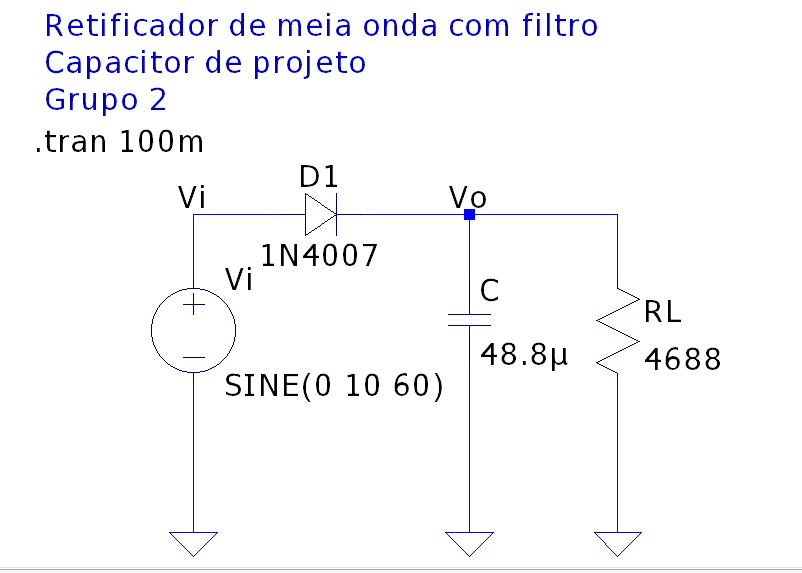
\includegraphics[width=0.85\textwidth]
    {imgs/simulacao/retificador_de_meia_onda_com_filtro_projeto.png}
    \caption{Circuito simulado do retificador de meia onda com filtro capacitivo.}
    \label{fig:sim_meia_onda_filtro}
\end{figure}

\begin{figure}[htbp]
    \centering
    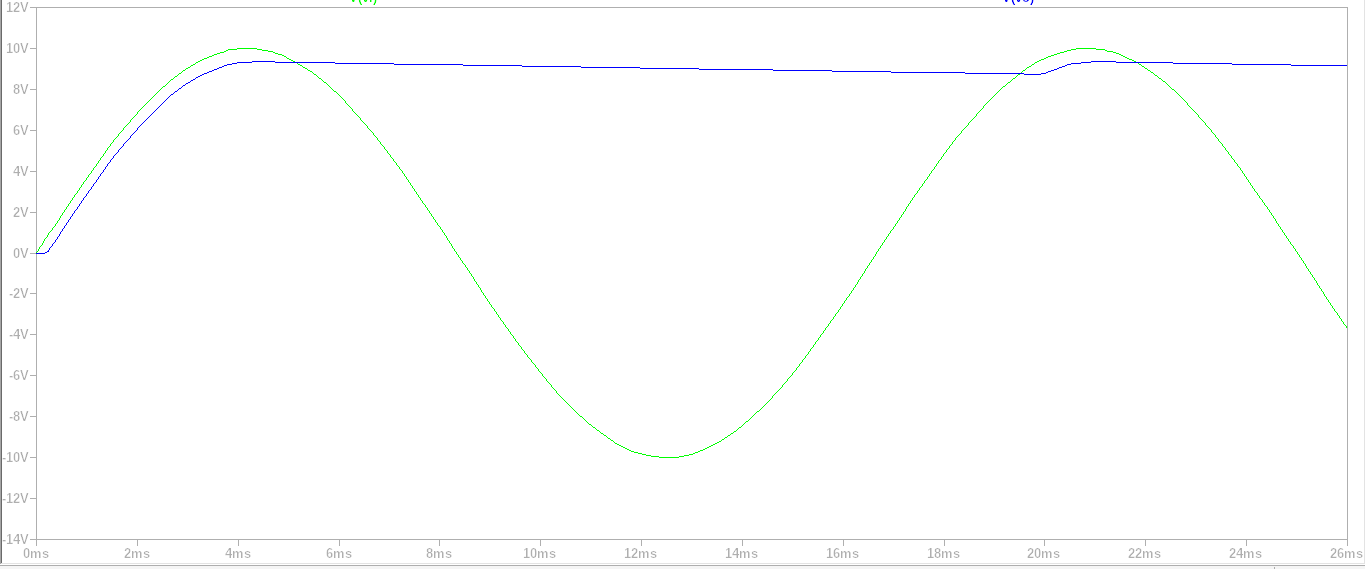
\includegraphics[width=0.85\textwidth]
    {imgs/simulacao/retificador_de_meia_onda_com_filtro_projeto_grafico.png}
    \caption{Formas de onda simuladas do retificador de meia onda com filtro.}
    \label{fig:sim_meia_onda_filtro_grafico}
\end{figure}

O ripple simulado foi de $0{,}60\,\text{V}_{pp}$, próximo dos $0{,}56\,\text{V}_{pp}$ medidos em bancada. A tensão contínua simulada foi de $9{,}1\,\text{V}$, superior aos $8{,}254\,\text{V}$ medidos. A diferença de tensão contínua pode estar relacionada à amplitude efetiva da fonte, ao comportamento de condução do diodo e à descarga do capacitor pela carga. Por esse motivo, a concordância entre os ripples não implica necessariamente igualdade entre as tensões médias.

A relação aproximada entre a corrente de carga, a frequência, a capacitância e o ripple é dada por

\[
V_r \approx \frac{I_L}{fC}.
\]

Essa expressão indica que o aumento da capacitância reduz a queda de tensão do capacitor entre picos sucessivos, desde que as demais condições permaneçam semelhantes.

\paragraph{Retificador de meia onda com o capacitor de comparação.}

Para avaliar o efeito da redução da capacitância, foi simulada a mesma configuração com o capacitor medido de $4{,}84\,\mu\text{F}$. As Figuras~\ref{fig:sim_meia_onda_comparacao} e~\ref{fig:sim_meia_onda_comparacao_grafico} apresentam o circuito e as formas de onda correspondentes.

\begin{figure}[htbp]
    \centering
    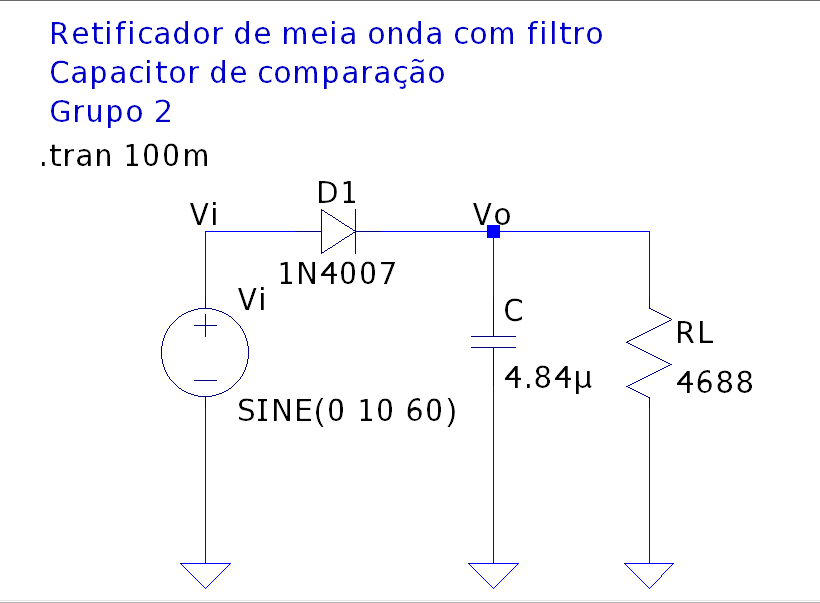
\includegraphics[width=0.85\textwidth]
    {imgs/simulacao/retificador_de_meia_onda_com_filtro_comparacao.png}
    \caption{Circuito simulado do retificador de meia onda com o capacitor de comparação.}
    \label{fig:sim_meia_onda_comparacao}
\end{figure}

\begin{figure}[htbp]
    \centering
    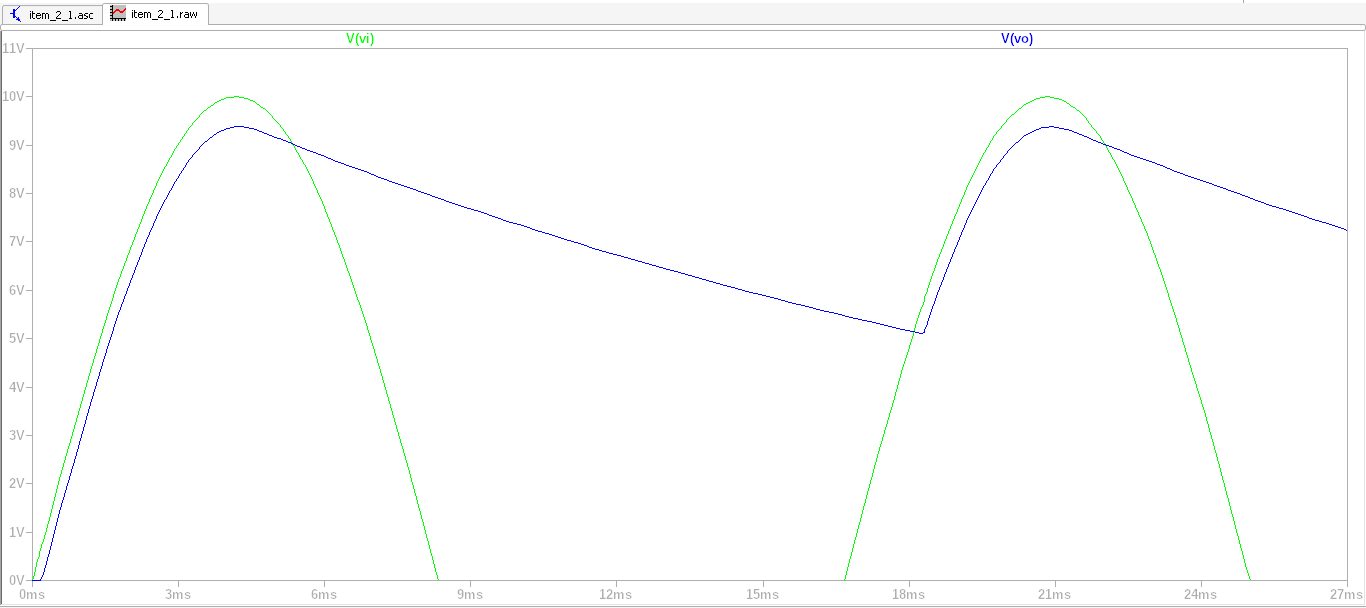
\includegraphics[width=0.85\textwidth]
    {imgs/simulacao/retificador_de_meia_onda_com_filtro_comparacao_grafico.png}
    \caption{Formas de onda simuladas com o capacitor de comparação.}
    \label{fig:sim_meia_onda_comparacao_grafico}
\end{figure}

Com o capacitor menor, o ripple simulado aumentou para $4{,}27\,\text{V}_{pp}$, e a tensão contínua simulada diminuiu para $7{,}12\,\text{V}$. Em bancada, foram registrados $4{,}16\,\text{V}_{pp}$ de ripple e $7{,}038\,\text{V}$ de tensão contínua. A proximidade entre os resultados simulados e medidos para essa configuração indica que o modelo reproduz satisfatoriamente o aumento da ondulação causado pela redução da capacitância.

A razão entre o ripple com o capacitor menor e o ripple com o capacitor principal foi de aproximadamente $7{,}13$ na simulação e $7{,}43$ na bancada. Esses resultados são próximos da razão entre as capacitâncias medidas, embora não sejam exatamente iguais, pois a expressão de ripple é uma aproximação e o circuito real possui condução não ideal dos diodos e intervalos de recarga finitos.

\paragraph{Ponte retificadora sem filtro.}

A ponte foi simulada com quatro diodos 1N4007, sem capacitor, e com a carga conectada à referência de saída. A Figura~\ref{fig:sim_ponte} apresenta o circuito simulado e a Figura~\ref{fig:sim_ponte_grafico} mostra as formas de onda obtidas.

\begin{figure}[htbp]
    \centering
    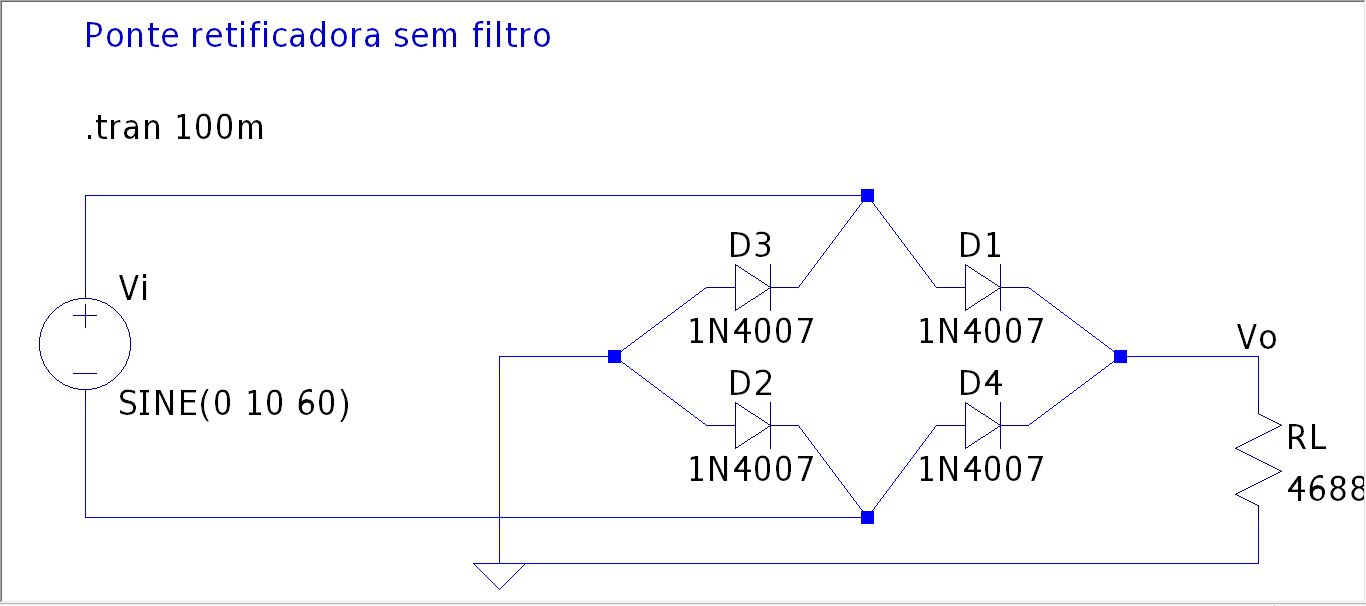
\includegraphics[width=0.85\textwidth]
    {imgs/simulacao/ponte_retificadora_sem_filtro.png}
    \caption{Circuito simulado da ponte retificadora sem filtro.}
    \label{fig:sim_ponte}
\end{figure}

\begin{figure}[htbp]
    \centering
    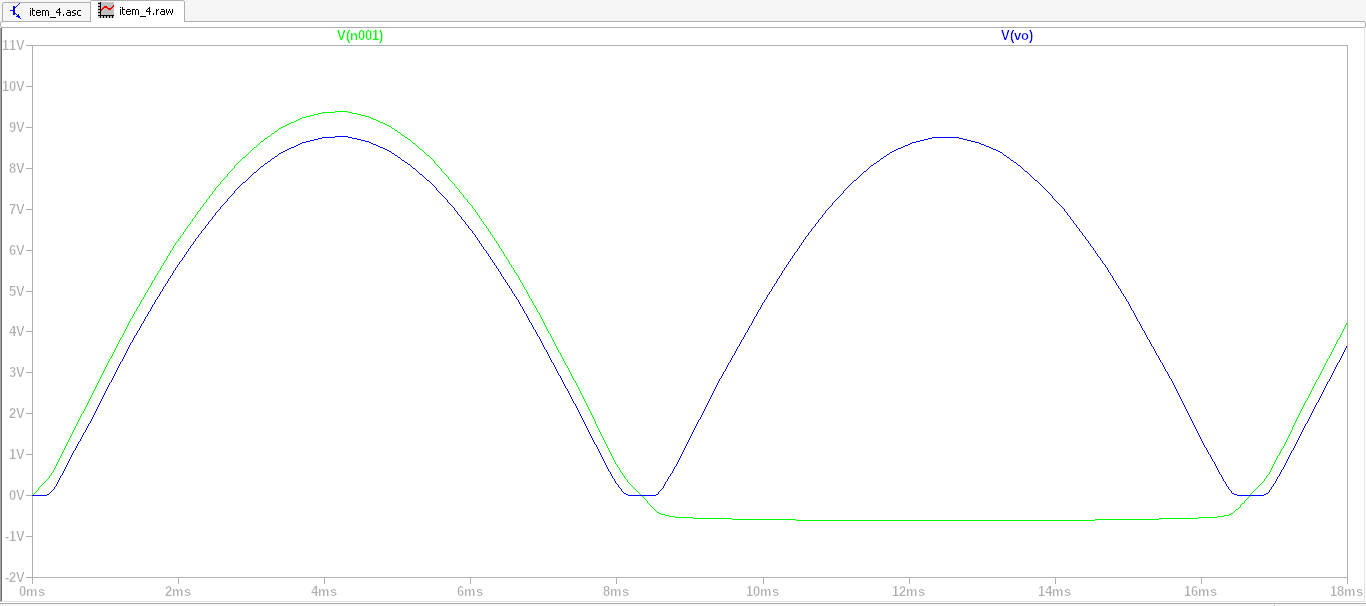
\includegraphics[width=0.85\textwidth]
    {imgs/simulacao/ponte_retificadora_sem_filtro_grafico.png}
    \caption{Formas de onda simuladas da ponte retificadora sem filtro.}
    \label{fig:sim_ponte_grafico}
\end{figure}

O pico simulado na saída foi de $8{,}7\,\text{V}$, correspondente a uma diferença de $1{,}3\,\text{V}$ em relação ao pico nominal de $10\,\text{V}$. Essa diferença é compatível com a condução de dois diodos em série no caminho da corrente. A frequência dos picos foi de $120\,\text{Hz}$, o dobro da frequência da fonte, pois os semiciclos positivos e negativos são convertidos em pulsos de mesma polaridade.

Na bancada, o pico de saída foi de $8{,}4\,\text{V}$ e a frequência medida foi de $119\,\text{Hz}$. A diferença de $1{,}6\,\text{V}$ em relação ao pico nominal foi superior à queda observada na montagem de meia onda, conforme esperado pela presença de dois diodos no caminho de condução.

\paragraph{Ponte retificadora com filtro capacitivo.}

Na simulação da ponte com filtro, foi conectado o capacitor de $48{,}8\,\mu\text{F}$ em paralelo com a carga. O capacitor é recarregado a cada semiciclo, fazendo com que a frequência dos picos de recarga seja de aproximadamente $120\,\text{Hz}$. Para uma mesma corrente de carga e capacitância, essa duplicação da frequência tende a reduzir o ripple em comparação com a retificação de meia onda.

As Figuras~\ref{fig:sim_ponte_filtro} e~\ref{fig:sim_ponte_filtro_grafico} apresentam o circuito e as formas de onda simuladas.

\begin{figure}[htbp]
    \centering
    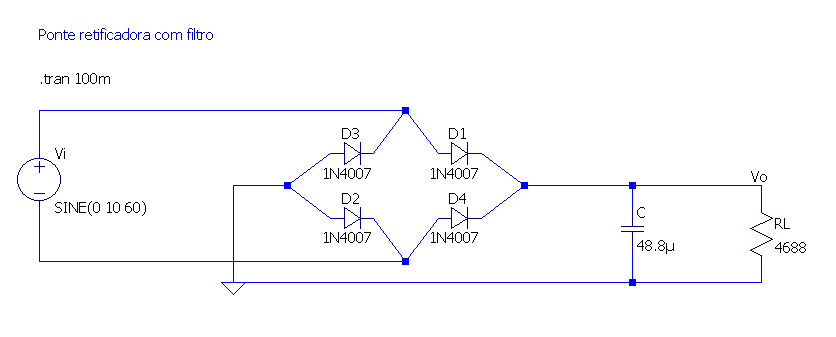
\includegraphics[width=0.85\textwidth]
    {imgs/simulacao/ponte_com_filtro.png}
    \caption{Circuito simulado da ponte retificadora com filtro capacitivo.}
    \label{fig:sim_ponte_filtro}
\end{figure}

\begin{figure}[htbp]
    \centering
    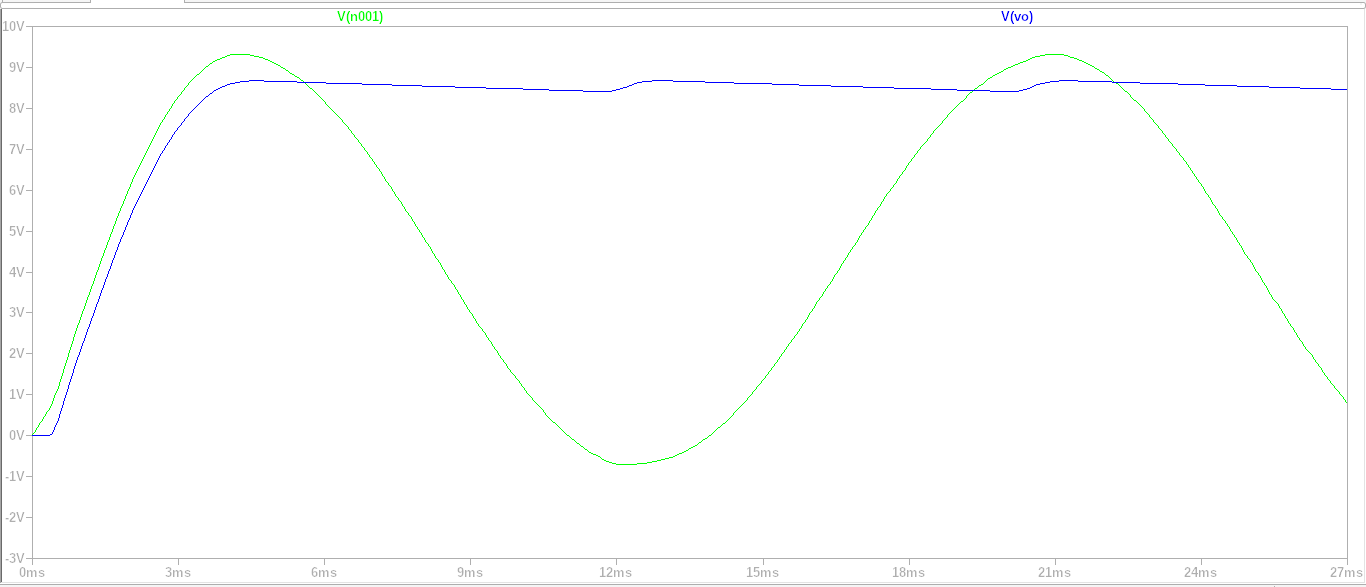
\includegraphics[width=0.85\textwidth]
    {imgs/simulacao/ponte_com_filtro_grafico.png}
    \caption{Formas de onda simuladas da ponte retificadora com filtro.}
    \label{fig:sim_ponte_filtro_grafico}
\end{figure}

O ripple simulado foi de $0{,}26\,\text{V}_{pp}$, igual ao valor registrado na bancada. A tensão contínua simulada foi de $8{,}0\,\text{V}$, enquanto a medida experimental foi de $8{,}004\,\text{V}$. Portanto, nessa configuração, houve boa concordância entre a simulação e a medição tanto para a ondulação quanto para a tensão contínua.

Considerando o ripple de $0{,}60\,\text{V}_{pp}$ da simulação de meia onda com o mesmo capacitor, a razão entre os ripples da ponte e do retificador de meia onda foi de aproximadamente $0{,}43$. Na bancada, a razão foi de

\[
\frac{V_{r,\mathrm{ponte}}}{V_{r,\mathrm{meia\ onda}}}
=
\frac{0{,}26}{0{,}56}
\approx 0{,}46.
\]

Ambos os resultados são próximos da razão teórica de $0{,}5$, prevista pela duplicação da frequência de recarga. A pequena diferença em relação ao valor ideal pode ser atribuída ao caráter aproximado do modelo de ripple e às diferenças entre as condições de condução e descarga nas duas montagens.

\paragraph{Regulação com zener.}

A última simulação acrescenta à ponte com filtro o resistor em série e o diodo zener em paralelo com a carga. O resistor limita a corrente total fornecida pelo filtro, que se divide entre a carga e o zener. Quando a corrente reversa no zener é suficiente para mantê-lo na região de ruptura, a tensão na carga permanece aproximadamente constante, mesmo com a ondulação presente na entrada do regulador.

A Figura~\ref{fig:sim_zener} apresenta o circuito de regulação, e a Figura~\ref{fig:sim_zener_grafico} apresenta os resultados transientes.

\begin{figure}[htbp]
    \centering
    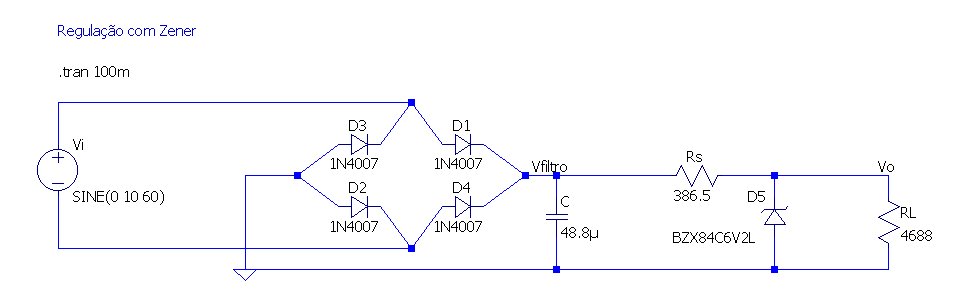
\includegraphics[width=0.85\textwidth]
    {imgs/simulacao/regulacao_com_zener.png}
    \caption{Circuito simulado da ponte com filtro e regulador zener.}
    \label{fig:sim_zener}
\end{figure}

\begin{figure}[htbp]
    \centering
    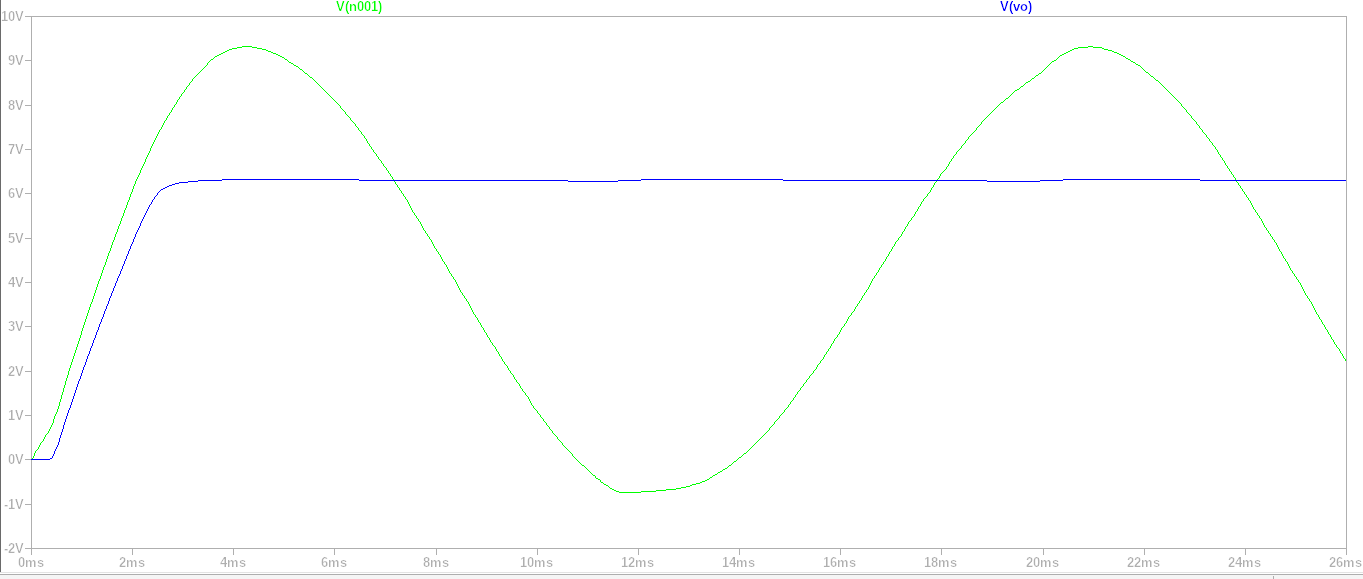
\includegraphics[width=0.85\textwidth]
    {imgs/simulacao/regulacao_com_zener_grafico.png}
    \caption{Formas de onda simuladas do regulador zener.}
    \label{fig:sim_zener_grafico}
\end{figure}

A planilha registra tensão contínua de $5{,}6\,\text{V}$ na saída regulada, tanto na simulação quanto na medição com a carga conectada. O ripple simulado foi de $0{,}03\,\text{V}_{pp}$, enquanto o medido foi de $0{,}02\,\text{V}_{pp}$. Tomando como referência o ripple de $0{,}26\,\text{V}_{pp}$ antes do regulador, a simulação indica redução de aproximadamente $88{,}5\%$, e a medição indica redução de aproximadamente $92{,}3\%$.

Esses resultados demonstram que o regulador reduziu significativamente a ondulação da saída. Entretanto, a tensão registrada de $5{,}6\,\text{V}$ não coincide com os $6{,}8\,\text{V}$ nominais do 1N754 especificado no roteiro. A identificação do modelo de zener utilizado na simulação e na bancada precisa ser conferida antes de concluir que a tensão regulada corresponde ao valor nominal previsto.

Com a carga retirada, a tensão contínua medida foi de $5{,}604\,\text{V}$. Esse resultado é próximo da tensão observada com a carga conectada, mostrando que a saída permaneceu praticamente constante nas duas condições registradas. A avaliação da corrente e da potência no zener deve, contudo, utilizar a tensão nominal e o modelo do componente efetivamente empregado, juntamente com o valor medido de $R_S$.

Em síntese, as simulações e as medições apresentam concordância particularmente boa para o ripple da ponte com filtro e para o aumento do ripple quando se reduz a capacitância no retificador de meia onda. As diferenças mais evidentes aparecem na tensão contínua da meia onda com o capacitor principal e na tensão nominal atribuída ao zener. A análise dessas divergências exige considerar a amplitude efetiva da fonte, as características não ideais dos diodos, os valores medidos dos componentes e a confirmação da identificação do zener utilizado.




% \begin{figure}[htb]
% \centering
% % \includegraphics[width=0.8\linewidth]{arquivo.png}
% \fbox{\parbox[c][3.2cm][c]{0.8\linewidth}{\centering\color{cinza}
%   substitua por \texttt{\textbackslash includegraphics}}}
% \caption{Legenda descritiva. Diga o que a figura mostra e o que nela é relevante, e não
% apenas o nome do circuito.}
% \label{fig:exemplo}
% \end{figure}

\section{Resultados}

% Apresente o que vocês obtiveram, em tabela sempre que houver mais de dois números. Use o
% número de algarismos significativos que a medição sustenta, e não todos os que o programa
% imprime. Para cada leitura de bancada, informe o instrumento e a incerteza.

% Guarde a interpretação para a seção seguinte: aqui vocês mostram o que encontraram.

\subsection{Projeto de cada integrante}

% Uma tabela por integrante, ou uma tabela única com uma coluna por integrante, confrontando
% o valor analítico e o simulado para cada grandeza pedida no roteiro.

\subsection{Circuito montado}

% Para cada grandeza, o que o projeto do integrante montado previa, o que a simulação com os
% valores medidos devolveu, e o que vocês mediram na bancada. É desta tabela que sai a
% discussão.

% \begin{center}
% \begin{tabular}{@{}lrrrr@{}}
% \toprule
% \textbf{Grandeza} & \textbf{Projeto} & \textbf{Sim. montagem} & \textbf{Medido} &
% \textbf{Erro} \\
% \midrule
% & & & & \\
% \bottomrule
% \end{tabular}
% \end{center}

\section{Discussão}

% Percorra as três comparações na ordem em que aparecem no quadro da Seção~4: a conta contra
% a simulação de projeto, esta contra a simulação da montagem, e esta contra a medição. Cada
% passo isola uma causa, e a discussão fica bem mais curta quando eles não se misturam.

% Compare também os projetos dos integrantes entre si. Como as especificações são diferentes,
% os resultados diferem, e mostrar que essa diferença é a que a teoria previa vale mais do
% que repetir três vezes a mesma análise.

% Sempre que uma divergência for maior do que a incerteza esperada, aponte uma causa concreta
% e diga como ela poderia ser reduzida. Vale, por exemplo, a tolerância do componente, a
% resistência série do indutor, a impedância de entrada do osciloscópio, a banda do
% amplificador ou a resolução da varredura.

% Quando previsto e obtido coincidirem, explique por que era esperado que coincidissem, e o
% que essa coincidência não permite concluir.

% Por fim, retome as hipóteses que vocês declararam na fundamentação e diga quais se
% confirmaram. Se algo observado contrariar a previsão, resolva a contradição aqui.

\section{Conclusão}

% Retome o objetivo que vocês anunciaram na introdução e responda se ele foi atingido,
% apoiando a resposta em um número. Aponte a principal limitação do que foi feito e o que
% ela impede de afirmar. Evite trazer resultado novo nesta seção.

\section{Referências}

\begin{referencias}
\item SEDRA, A.~S.; SMITH, K.~C. \emph{Microeletrônica}. 5.~ed. São Paulo: Pearson
      Prentice Hall, 2007.
\item BOYLESTAD, R.~L.; NASHELSKY, L. \emph{Dispositivos Eletrônicos e Teoria de
      Circuitos}. 11.~ed. São Paulo: Pearson Education do Brasil, 2013.
\end{referencias}

\end{document}
